\documentclass{beamer}
%\documentclass[handout,t]{beamer}

\batchmode
% \usepackage{pgfpages}
% \pgfpagesuselayout{4 on 1}[letterpaper,landscape,border shrink=5mm]

\usepackage{amsmath,amssymb,enumerate,epsfig,bbm,calc,color,ifthen,capt-of}

\usetheme{Berlin}
\usecolortheme{bear}

\title{Combinatorial and Geometric Structure in the Self-Assembly of Polyhedra}
\author{Daniel Johnson}
%\date{\today}
%\date{April 15, 2015}
\date{March 26, 2015}
\pgfdeclareimage[height=1cm]{brown-logo}{brown-logo.pdf}
\logo{\pgfuseimage{brown-logo}\hspace*{0.3cm}}

\AtBeginSection[]
{
  \begin{frame}<beamer>
    \frametitle{Outline}
    \tableofcontents[currentsection]
  \end{frame}
}
\beamerdefaultoverlayspecification{<+->}
% -----------------------------------------------------------------------------
\begin{document}
% -----------------------------------------------------------------------------

\frame{\titlepage}

\section[Outline]{}
\begin{frame}{Outline}
  \tableofcontents
\end{frame}
% -----------------------------------------------------------------------------
% -----------------------------------------------------------------------------
\section{Introduction}
\subsection{Polyhedra}
\begin{frame}{What is a Polyhedron?}
\end{frame}
% -----------------------------------------------------------------------------
\begin{frame}{Classes of Polyhedra}
\end{frame}
% -----------------------------------------------------------------------------
\subsection{Scientific Motivation}
\begin{frame}{Viral Capsids}
\begin{columns}
    \begin{column}{0.48\textwidth}

    \end{column}
    \begin{column}{0.48\textwidth}
    \scalebox{0.19}{
      \begin{figure}
        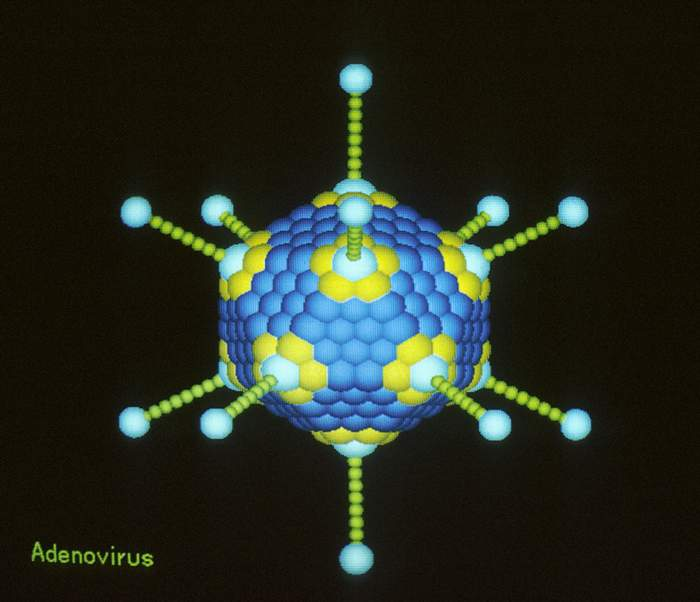
\includegraphics{Adenovirus.jpg}
        %\hspace*{15pt}\hbox{\scriptsize Credit:\thinspace{\small\itshape National Cancer Institute}}
        %\caption{Credit: National Cancer Institute}
       \end{figure}
     }
    \end{column}
\end{columns}
\end{frame}
% -----------------------------------------------------------------------------
\begin{frame}{Molecular Cages}
\begin{columns}
    \begin{column}{0.48\textwidth}

    \end{column}
    \begin{column}{0.48\textwidth}
    \scalebox{0.1}{
      \begin{figure}
        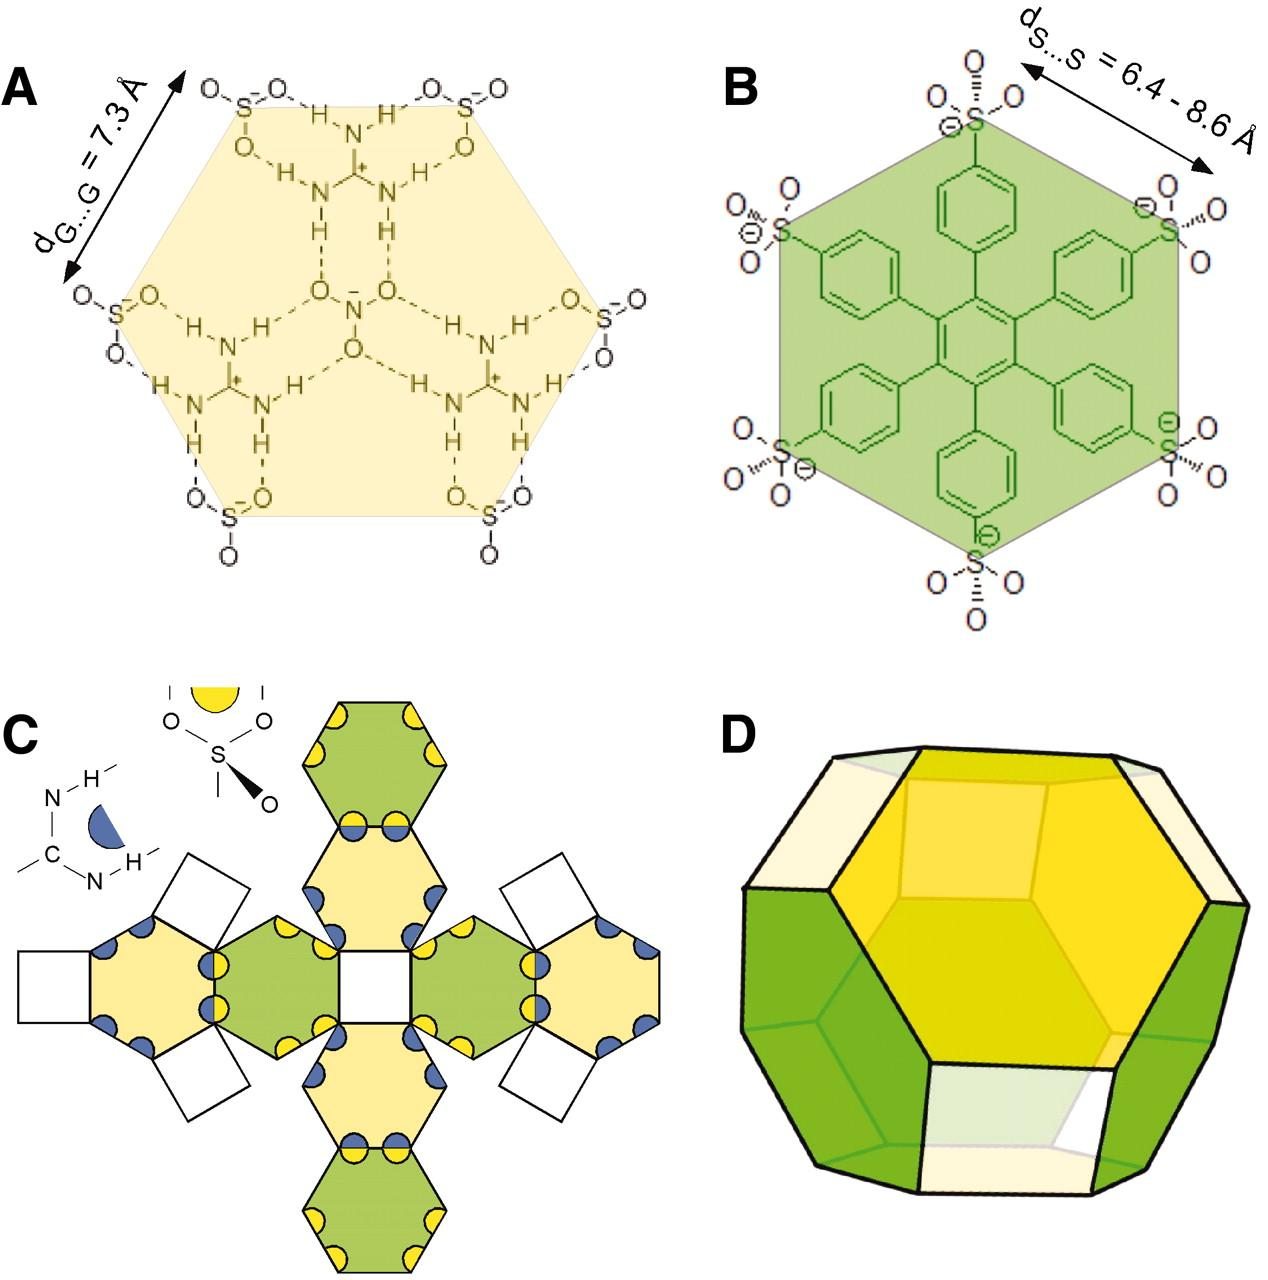
\includegraphics{ward_cage.png}
        %\hspace*{15pt}\hbox{\scriptsize Credit:\thinspace{\small\itshape National Cancer Institute}}
        %\caption{Credit: National Cancer Institute}
       \end{figure}
      }
    \end{column}
\end{columns}
\end{frame}
% -----------------------------------------------------------------------------
\begin{frame}{Self-Folding Polyhedra}
\end{frame}
% -----------------------------------------------------------------------------
\begin{frame}{Other Applications}
\begin{columns}
    \begin{column}{0.48\textwidth}
%        \includegraphics[width=<X>\textwidth]{}
\scalebox{0.19}{
        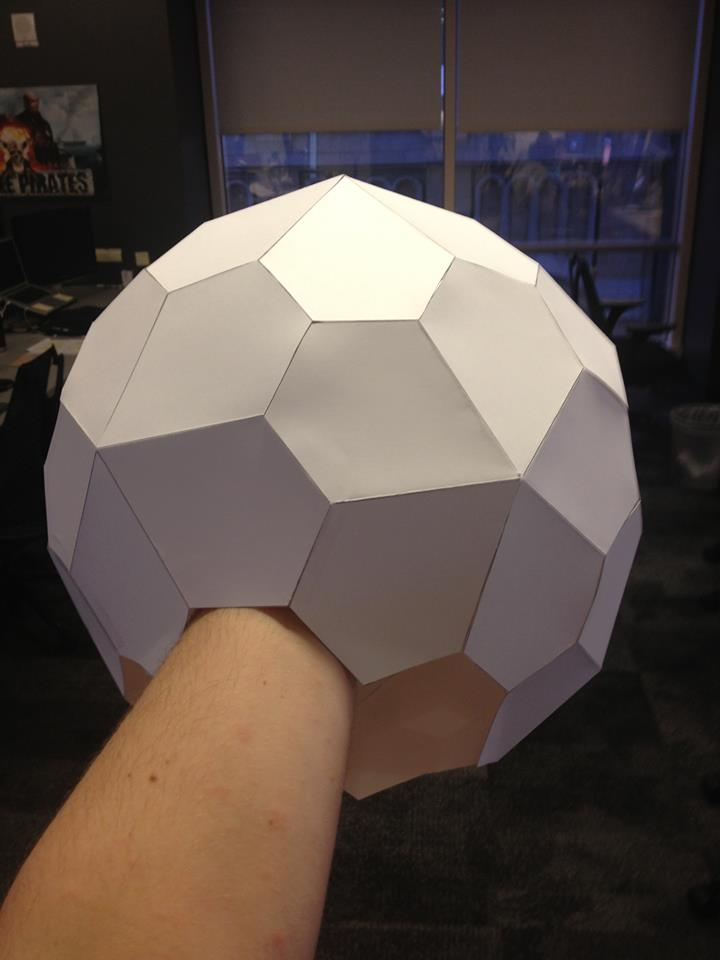
\includegraphics{jeremy_polyhedra.jpg}
}
    \end{column}
    \begin{column}{0.48\textwidth}
\scalebox{0.19}{
        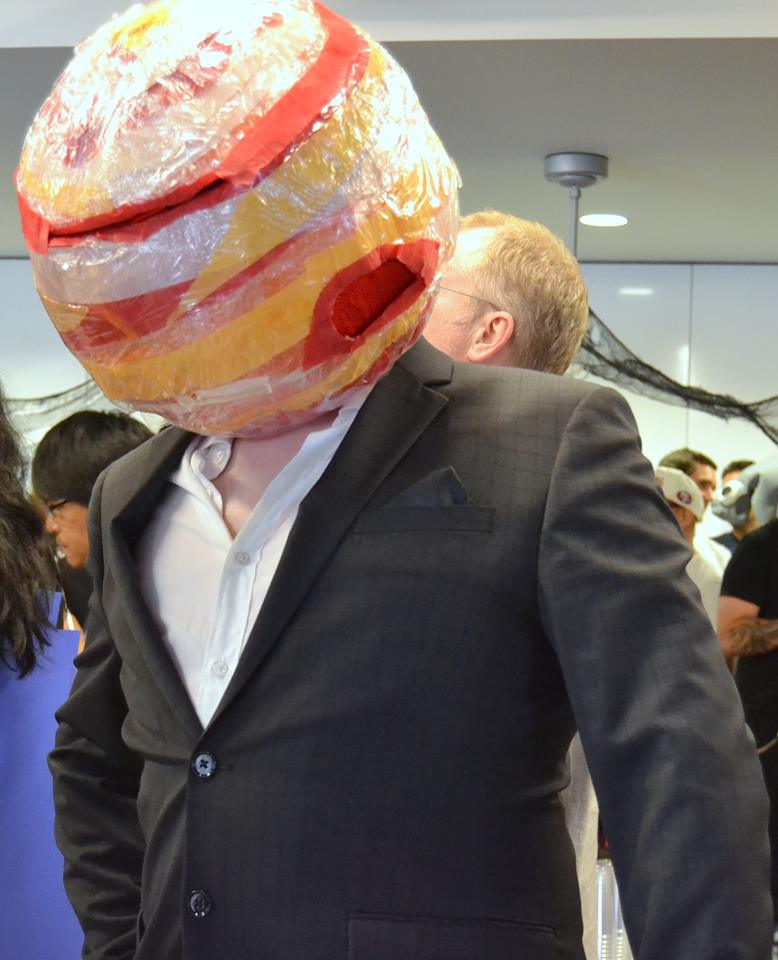
\includegraphics{mr_jupiter.jpg}
}
    \end{column}
\end{columns}
\end{frame}
% -----------------------------------------------------------------------------
% -----------------------------------------------------------------------------
\section{The Building Game: Modeling}
\subsection{Definitions}
\begin{frame}{The Building Game}
\begin{columns}
    \begin{column}{0.48\textwidth}

    \end{column}
    \begin{column}{0.48\textwidth}
    \scalebox{0.25}{
      \begin{figure}
        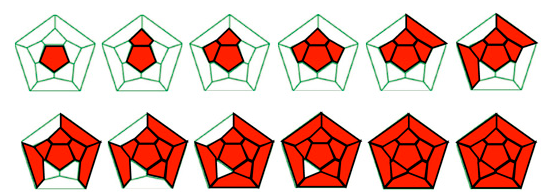
\includegraphics{bg.png}
        %\hspace*{15pt}\hbox{\scriptsize Credit:\thinspace{\small\itshape National Cancer Institute}}
        %\caption{Credit: National Cancer Institute}
       \end{figure}
      }
    \end{column}
\end{columns}
\end{frame}
% -----------------------------------------------------------------------------
\begin{frame}{States and Intermediates}
\begin{definition}
  A Building Game \textbf{state} $x \subset F$ is a non-empty subset of the faces $F$ of a polyhedron such that the the subset is connected along edges. 
\end{definition} 
\begin{definition}
A Building Game \textbf{intermediate} $[x]$ is an equivalence class on states given by the equivalence relation: $x \sim \hat{x}$ if $x$ can be rotated to get $\hat{x}$.
\end{definition}

\end{frame}
% -----------------------------------------------------------------------------
\begin{frame}{Connections and Degeneracies}
\end{frame}
% -----------------------------------------------------------------------------
\begin{frame}{Combinatorial Configuration Space}
\end{frame}
% -----------------------------------------------------------------------------
\begin{frame}{Pathways}
\end{frame}
% -----------------------------------------------------------------------------
\subsection{Stochastic Modeling} 
\begin{frame}{Markov Processes}
\end{frame}
% -----------------------------------------------------------------------------

\begin{frame}{Energetic Model}
\end{frame}
% -----------------------------------------------------------------------------

\begin{frame}{Stationary Distribution}
\begin{theorem}
The Markov process $X_t$ with rate matrix $Q$ has stationary distribution $\pi$.
$$\pi_j &= \frac{1}{zr_j}e^{-\beta E_j}$$
\end{theorem}
\begin{lemma}
$$ r_jS_{kj} = r_{k}S_{jk}$$
\end{lemma}
\end{frame}
% -----------------------------------------------------------------------------
\begin{frame}{Stationary Distribution II}
\begin{proof}
Detailed Balance!
\begin{align}
\pi_jQ_{jk} &= \left(\frac{1}{zr_j}e^{-\beta E_j}\right)\left(S_{jk}e^{-\beta\left(E_{jk} - E_j\right)}\right) \\
&= \left(\frac{1}{z}e^{-\beta E_{jk}}\right)\left(\frac{S_{jk}}{r_j}\right) \\
&= \left(\frac{1}{z}e^{-\beta E_{kj}}\right)\left(\frac{S_{kj}}{r_k}\right) \\
&= \pi_kQ_{kj}
\end{align}
\end{proof}
\end{frame}
% -----------------------------------------------------------------------------
\begin{frame}{Formation Times}
$$\tau_{j} &\doteq \inf\left\{t \geq 0 : X_t = [F], X_0 = [x^j]\right\}$$
\end{frame}
% -----------------------------------------------------------------------------
% -----------------------------------------------------------------------------
\section{The Building Game: Enumeration}
\subsection{Configuration Space Enumeration}
\begin{frame}{Configuration Space Statistics}
\begin{figure}[ht]
\scalebox{0.5}{
%{\footnotesize
\centering
%\textbf{Building Game Enumerative Results for the Platonic Solids}
\begin{tabular}{ l | c | r | r | r}
Polyhedra Name & $|F|$ & Intermediates & Connections & Pathways \\
  \hline    
Tetrahedron                     & 4        & 4     	& 3             & 1\\
Cube                            & 6        & 8     	& 9    		& 3\\
Octahedron                      & 8        & 14    	& 21    	& 14\\
Dodecahedron                    & 12       & 73    	& 263   	& 17,696 \\
Icosahedron                     & 20       & 2,649 	& 17,241        & 57,396,146,640\\ \hline
Truncated Tetrahedron           & 8     & 28    	& 63            & 402\\
Cuboctahedron                   & 14  	& 340   	& 1,634         & 10,170,968\\
Truncated Cube                  & 14  	& 499   	& 2,729         & 101,443,338 \\
Truncated Octahedron            & 14  	& 555           & 3,069         & 68,106,377\\
Rhombicuboctahedron             & 26  	& 638,850       & 6,459,801     & 164,068,345,221,515,292,308\\
Truncated Cuboctahedron         & 26  	& 1,525,658     & 17,672,374    & 13,837,219,462,483,379,105,902\\ \hline  
Triakis Tetrahedron             & 12  	& 98            & 318           & 38,938\\
Rhombic Dodecahedron            & 12  	& 127           & 493           & 76,936\\
Triakis Octahedron              & 24  	& 12,748        & 81,296        & 169,402,670,046,670\\
Tetrakis Hexahedron             & 24  	& 50,767        & 394,377       & 4,253,948,297,210,346\\
Deltoidal Icositetrahedron      & 24  	& 209,675       & 1,989,548     & 418,663,242,727,526,726 \\
Pentagonal Icositetrahedron     & 24  	& 345,938       & 3,544,987     & 2,828,128,000,716,774,492\\
Rhombic Triacontahedron         & 30  	& 2,423,212     & 26,823,095    & 161,598,744,916,797,017,978,128\\
\end{tabular}
}
%\caption{Building game combinatorial configuration space enumerative results for the Platonic, Archimedean, and Catalan solids.}
\label{tab:bgEnum}
\end{figure}

\end{frame}
% -----------------------------------------------------------------------------

\begin{frame}{Computation}
\begin{itemize}

\end{itemize}
\end{frame}
% -----------------------------------------------------------------------------

\subsection{Shellings}
\begin{frame}{Shellings and Shellability}
\begin{figure}[ht]
\scalebox{0.6}{
%{\footnotesize
\centering
%\textbf{Building Game Enumerative Results for the Platonic Solids}
\begin{tabular}{ l | c | r}
Polyhedra Name & $|F|$ & Shellings \\
  \hline    
Tetrahedron                     & 4  	& 24 \\                         
Cube                            & 6  	& 480 \\                        
Octahedron                      & 8  	& 4,224\\                       
Dodecahedron                    & 12 	& 19,041,600 \\                 
Icosahedron                     & 20 	& 1,417,229,099,520 \\ \hline   
Truncated Tetrahedron           & 8     & 9,216 \\                      
Cuboctahedron                   & 14	& 113,055,744 \\                
Truncated Cube                  & 14	& 654,801,408 \\                
Truncated Octahedron            & 14	& 937,087,104 \\                
Rhombicuboctahedron             & 26	& 4,728,400,467,971,102,208 \\  
Truncated Cuboctahedron         & 26	& 688,499,026,944,479,645,952 \\ \hline
Triakis Tetrahedron             & 12    & 587,040\\                     
Rhombic Dodecahedron            & 12 	& 5,836,800\\                   
Triakis Octahedron              & 24	& 66,063,419,534,592 \\         
Tetrakis Hexahedron             & 24	& 1,389,323,257,015,296 \\      
Deltoidal Icositetrahedron      & 24	& 125,987,819,253,281,472\\     
Pentagonal Icositetrahedron     & 24	& 1,144,572,832,023,047,616 \\  
Rhombic Triacontahedron         & 30	& 15,574,782,555,813,226,074,240 \\
\end{tabular}
}
%\caption{Number of Shellings for the Platonic, Archimedean, and Catalan solids of up to 30 faces.}
\label{tab:Shellings}
\end{figure}

\end{frame}
% -----------------------------------------------------------------------------
\begin{frame}{Computation}
\end{frame}
% -----------------------------------------------------------------------------
% -----------------------------------------------------------------------------
\section{Conclusions}
\begin{frame}{Summary}
\end{frame}
% -----------------------------------------------------------------------------
\begin{frame}{Acknowledgements}
\end{frame}


\end{document}
% -----------------------------------------------------------------------------
% -----------------------------------------------------------------------------
% -----------------------------------------------------------------------------
% -----------------------------------------------------------------------------
% -----------------------------------------------------------------------------
\section{Introduction}
\subsection{Cracked Pots -- an uncharted field}
\begin{frame}{Why study Psychoceramics?}
  \begin{itemize}
    \item Plenty of subjects available for study
    \item Bright Job Prospects
    \item Ample Funding (Josiah S. Carberry Fund)
  \end{itemize}
\end{frame}
\begin{frame}{Past Work}
  Work done by JSC:
  \pause
  \begin{itemize}
    \item<2-> Archaic Greek Architectural Revetments in Connection with Ionian Philology
    \item<3-> Another Catullus to Another Lesbia
  \end{itemize}
  \pause[4]
  Work done by Others:
  \begin{itemize}
    \item<5-> Nothing
  \end{itemize}
  
\end{frame}
% -----------------------------------------------------------------------------
\section{Conclusions}
\subsection{Additional Aspects}
\begin{frame}{Questions and Answers}
  More Questions?

  \begin{itemize}
    \item Browse \url{http://tinyurl.com/43dwrt}.
    \item Contact my assistant Truman Grayson.
  \end{itemize}
  
\end{frame}
% -----------------------------------------------------------------------------


